\documentclass{article}\usepackage[]{graphicx}\usepackage[]{xcolor}
% maxwidth is the original width if it is less than linewidth
% otherwise use linewidth (to make sure the graphics do not exceed the margin)
\makeatletter
\def\maxwidth{ %
  \ifdim\Gin@nat@width>\linewidth
    \linewidth
  \else
    \Gin@nat@width
  \fi
}
\makeatother

\definecolor{fgcolor}{rgb}{0.345, 0.345, 0.345}
\newcommand{\hlnum}[1]{\textcolor[rgb]{0.686,0.059,0.569}{#1}}%
\newcommand{\hlsng}[1]{\textcolor[rgb]{0.192,0.494,0.8}{#1}}%
\newcommand{\hlcom}[1]{\textcolor[rgb]{0.678,0.584,0.686}{\textit{#1}}}%
\newcommand{\hlopt}[1]{\textcolor[rgb]{0,0,0}{#1}}%
\newcommand{\hldef}[1]{\textcolor[rgb]{0.345,0.345,0.345}{#1}}%
\newcommand{\hlkwa}[1]{\textcolor[rgb]{0.161,0.373,0.58}{\textbf{#1}}}%
\newcommand{\hlkwb}[1]{\textcolor[rgb]{0.69,0.353,0.396}{#1}}%
\newcommand{\hlkwc}[1]{\textcolor[rgb]{0.333,0.667,0.333}{#1}}%
\newcommand{\hlkwd}[1]{\textcolor[rgb]{0.737,0.353,0.396}{\textbf{#1}}}%
\let\hlipl\hlkwb

\usepackage{framed}
\makeatletter
\newenvironment{kframe}{%
 \def\at@end@of@kframe{}%
 \ifinner\ifhmode%
  \def\at@end@of@kframe{\end{minipage}}%
  \begin{minipage}{\columnwidth}%
 \fi\fi%
 \def\FrameCommand##1{\hskip\@totalleftmargin \hskip-\fboxsep
 \colorbox{shadecolor}{##1}\hskip-\fboxsep
     % There is no \\@totalrightmargin, so:
     \hskip-\linewidth \hskip-\@totalleftmargin \hskip\columnwidth}%
 \MakeFramed {\advance\hsize-\width
   \@totalleftmargin\z@ \linewidth\hsize
   \@setminipage}}%
 {\par\unskip\endMakeFramed%
 \at@end@of@kframe}
\makeatother

\definecolor{shadecolor}{rgb}{.97, .97, .97}
\definecolor{messagecolor}{rgb}{0, 0, 0}
\definecolor{warningcolor}{rgb}{1, 0, 1}
\definecolor{errorcolor}{rgb}{1, 0, 0}
\newenvironment{knitrout}{}{} % an empty environment to be redefined in TeX

\usepackage{alltt}
\usepackage{amsmath} %This allows me to use the align functionality.
                     %If you find yourself trying to replicate
                     %something you found online, ensure you're
                     %loading the necessary packages!
\usepackage{amsfonts}%Math font
\usepackage{graphicx}%For including graphics
\usepackage{hyperref}%For Hyperlinks
\usepackage[shortlabels]{enumitem}% For enumerated lists with labels specified
                                  % We had to run tlmgr_install("enumitem") in R
\hypersetup{colorlinks = true,citecolor=black} %set citations to have black (not green) color
\usepackage{natbib}        %For the bibliography
\setlength{\bibsep}{0pt plus 0.3ex}
\bibliographystyle{apalike}%For the bibliography
\usepackage[margin=0.50in]{geometry}
\usepackage{float}
\usepackage{multicol}

%fix for figures
\usepackage{caption}
\newenvironment{Figure}
  {\par\medskip\noindent\minipage{\linewidth}}
  {\endminipage\par\medskip}
\IfFileExists{upquote.sty}{\usepackage{upquote}}{}
\begin{document}

\vspace{-1in}
\title{Lab 10 -- MATH 240 -- Computational Statistics}

\author{
  Reagan Sernick \\
  {\tt rsernick@colgate.edu}
}

\date{04/09/25}

\maketitle

\begin{multicols}{2}
%\raggedcolumns % If your spacing gets messed up try uncommenting 
                % this line

\noindent \textbf{Keywords:} \textbf{Binomial Distribution:} a probability distribution that summarizes the likelihood of a given number of successes in a fixed number of independent trials, each with the same probability of success.
; \textbf{Margin of Error (MOE):} range of values above and below a sample statistic that is likely to contain the true population parameter, given a certain confidence level.

\section{Introduction}

This report explores the relationship between binomial distributions and margin of error in the context of political polling data. Using simulations and resampling methods based on a Gallup poll, we examine how changes in sample size and population proportion affect the variability of survey estimates. By modeling the sampling distribution with binomial assumptions, we highlight how statistical tools can quantify uncertainty and improve confidence in public opinion measurements.

\section{Methods}

The data we use in this lab came from a Gallup polls political poll of 1004 randomly sampled Americans. Gallup reported that 39\% of respondents were satisfied with the position of the United States in the world today, 59\% were not, and 2\% had no opinion. They also reported a 4\% margin of error and claimed that if the sample size were doubled the MOE would be halved.

\subsection{Simulation Assuming the Value of p}

If we assume the value of p to be $\hat{p}$ (0.39) we can use \texttt{rbinom()} to simulate a sampling distribution at any given sample size.

\subsubsection{Sample size of 1004}

For this task we ran a simulation of 10,000 samples of size 1004, to see what a sampling distribution might look like if the population parameter p was 0.39.

\begin{figure}[H]
\label{p1}
\centering
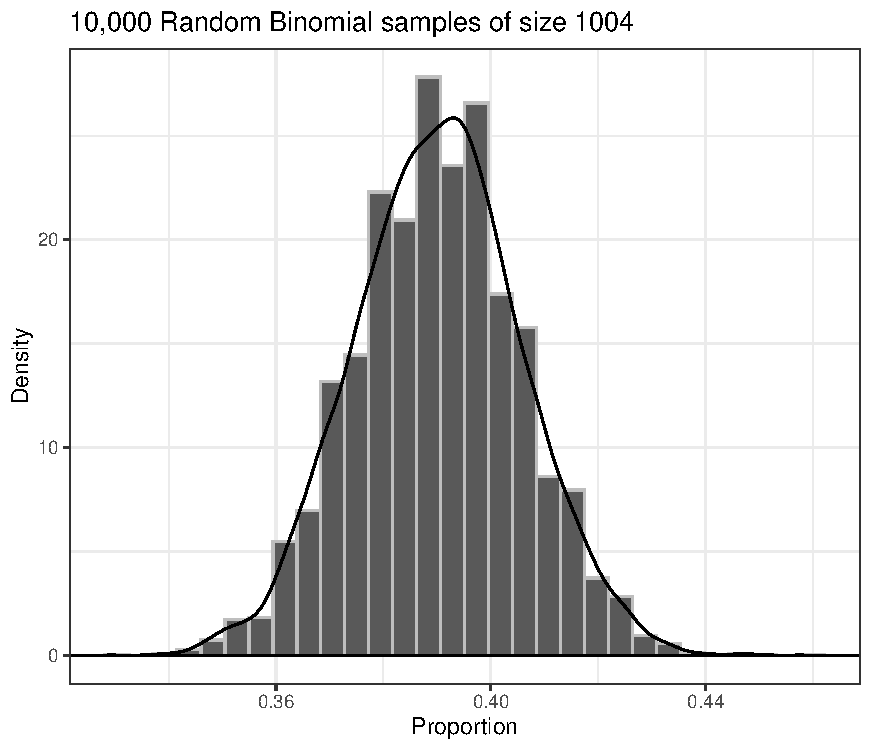
\includegraphics[width=2.5in]{rbin_1004.pdf}
\caption{Sampling distribution of sample size 1004}
\end{figure}

\subsubsection{Sample size of 2008}

Much like the last task, we ran a simulation of 10,000 samples  assuming p to be 0.39, but doubled the sample size to be 2008.

\begin{figure}[H]
\label{p2}
\centering
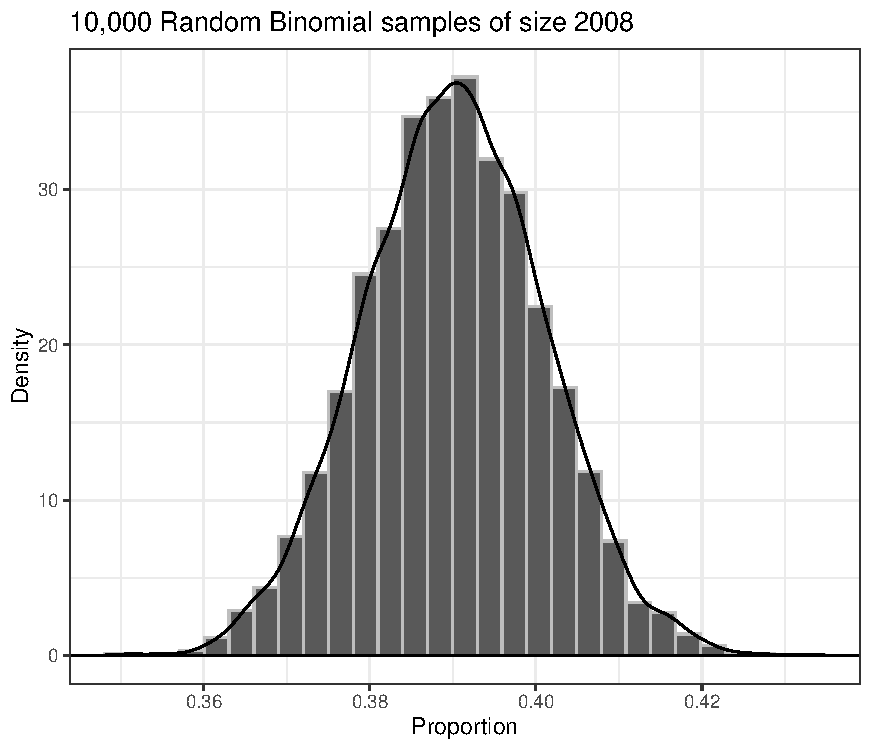
\includegraphics[width=2.5in]{rbin_2008.pdf}
\caption{Sampling distribution of sample size 2008}
\end{figure}

This graph shows significantly less variation than the previous one, and appears to be more normally distributed as well. 

\subsection{Simulation Without Knowing the Value of p}

While \texttt{rbinom()} can help create a realistic sampling distribution based on the parameter p, it is not often that we know the value of the population parameter. In this case it would make more sense to use resampling. However, in order to do resampling, some conditions must be met:

\begin{description}
  \item[Approximately Gaussian] Sample size (1004) $>$ 30 so Central Limit Theorem (CLT) applies
  \item[Representative] The researchers performed this survey carefully to make sure that the sample is representative
\end{description}

Knowing the conditions were met I was able to resample the data using \texttt{sample()} on sample data I created from the given proportions. 

\begin{figure}[H]
\label{p3}
\centering
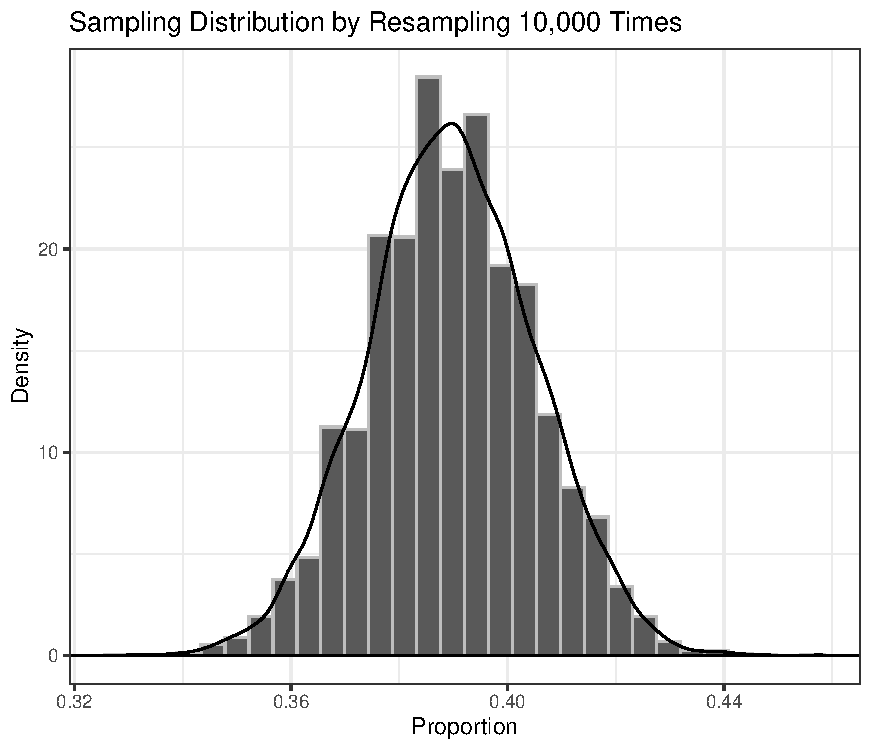
\includegraphics[width=2.5in]{resample.pdf}
\caption{Resample from original sample of size 1004}
\end{figure}


\subsection{How do n and p Affect Margin of Error?}

In order to see how both sample size and the probability parameter affect MOE, we ran a simulation across n in \{100, 110, 120, ..., 3000\} and p in \{0.01, 0.02, ..., 0.99\}. This simulation was the same as the first 2, 10,000 samples using \texttt{rbinom()}, but n and p were varied. For this complicated simulation we generated $2,900*99*10,000 = 2,871,000,000$ random responses. This method was used once for our MOE estimate (half the range of the middle 95\%) and once for Wilson's MOE:

\[
\frac{z_{1 - \alpha/2} \sqrt{n\hat{p}(1 - \hat{p}) + \frac{z_{1 - \alpha/2}^2}{4}}}{n + z_{1 - \alpha/2}^2}
\]

\section{Results}

\subsection{Does Resampling Work?}

The theory behind resampling is that if the conditions are met, as n (number of resamples) gets larger the resampled sampling distribution tends towards a sampling distribution of n samples the same size. The Gallup poll data meets the conditions for resampling so our resampled distribution should be close to a random sampling distribution. This is exactly what we see in \hyperref[p1]{Figure 1} and \hyperref[p3]{Figure 3}, the distribution of the \texttt{rbinom()} data and the resample are almost identical.

\begin{table}[H]
\centering
\begin{tabular}{rlr}
  \hline
 & Sample & MOE \\ 
  \hline
  1 & rbinom size 1004 & 0.02988048 \\ 
  2 & rbinom size 2008 & 0.02116534 \\ 
  3 & resample & 0.02988048 \\ 
   \hline
\end{tabular}
\caption{Estimated MOEs for simulations}
\end{table}

Furthermore, as seen in Table 1 above, the margin of error of the first simulation and the resampling distribution are identical to 8 decimal places.

\subsection{Relationship between n, p and MOE}

Both margin of error raster plots seen in \hyperref[p4]{Figure 4} reveal interesting details about MOE as a function of n and p. The first thing I noticed is that at the extremes of p (near 1 and 0), and any value of n, MOE is low. Another detail is that the largest MOE is at p = 0.50 for every value of n. This relationship can be generalized to as n increases MOE increases, and as p gets further from 0.50 in any direction MOE increases.

Additionally, \hyperref[p4]{Figure 4} reveals the accuracy of our MOE estimate compared to Wilson's MOE. The MOE estimate plot is noisy, meaning it is slightly imprecise, but the Wilson's MOE is significantly less noisy, meaning it is much more precise.



%%%%%%%%%%%%%%%%%%%%%%%%%%%%%%%%%%%%%%%%%%%%%%%%%%%%%%%%%%%%%%%%%%%%%%%%%%%%%%%%
% Bibliography
%%%%%%%%%%%%%%%%%%%%%%%%%%%%%%%%%%%%%%%%%%%%%%%%%%%%%%%%%%%%%%%%%%%%%%%%%%%%%%%%
\vspace{2em}


\begin{tiny}
\bibliography{bib}
\end{tiny}
\end{multicols}

%%%%%%%%%%%%%%%%%%%%%%%%%%%%%%%%%%%%%%%%%%%%%%%%%%%%%%%%%%%%%%%%%%%%%%%%%%%%%%%%
% Appendix
%%%%%%%%%%%%%%%%%%%%%%%%%%%%%%%%%%%%%%%%%%%%%%%%%%%%%%%%%%%%%%%%%%%%%%%%%%%%%%%%
\newpage
\onecolumn
\section{Appendix}

\begin{figure}[ht]
\label{p4}
\centering
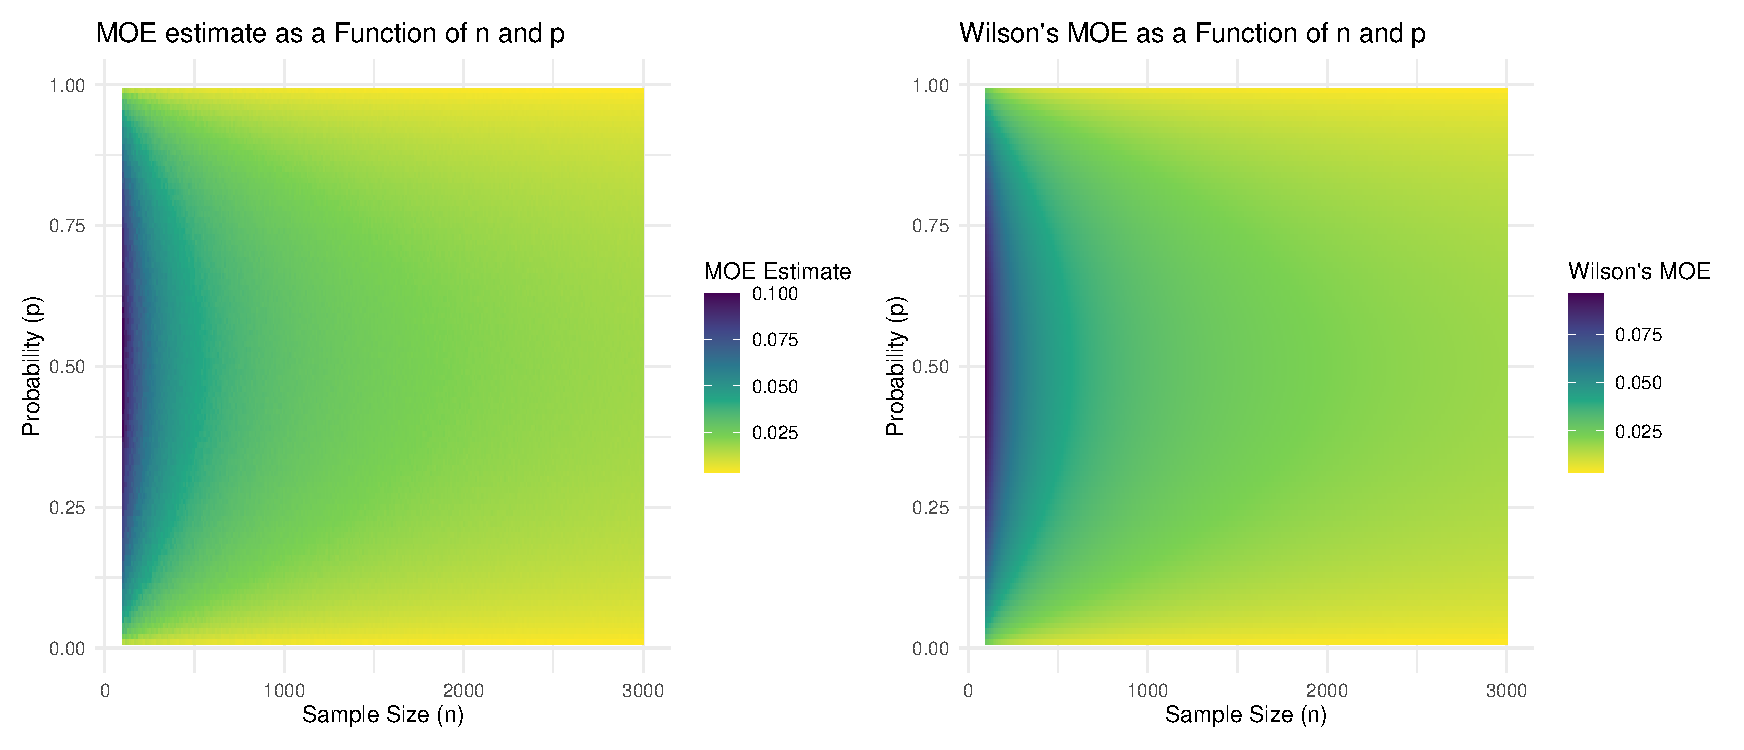
\includegraphics[width=\linewidth]{w+e.pdf}
\caption{Combined raster plots of MOE estimates and Wilson's MOE (\emph{I reversed the colors because it makes more sense to me this way})}
\end{figure}

\end{document}
